\chapter{Space-Time DPG on Parabolic Equations}



\section{Abstract parabolic equation}

Let $V$ and $H$ be separable Hilbert spaces such that $V\hookrightarrow H$ with dense compact embedding. Identifying $H$ with its dual, we obtain the Gelfand triple $V\hookrightarrow H\simeq H'\hookrightarrow V'$. For almost all $t\in \mathcal{I}=(0,T)\subset\R$, let $a(t;\bdot,\bdot)$ be a bilinear form on $V\times V$ such that for any $\mu,\lambda\in V$, $t\rightarrow a(t;\mu,\lambda)$ is measurable on $\mathcal{I}$, and such that for some constant $\delta\geq0$, for almost every $t\in\mathcal{I}$, and all $\lambda,\mu$,

\begin{align*}
    |a(t;\mu,\lambda)|&\lesssim\norm{\mu}_V\norm{\lambda}_V \text{ (boundedness),}\\
    a(t;\mu,\mu)+\delta\norm{\mu}_V^2&\gtrsim \norm{\mu}_V^2 \text{ (Gårding inequality).}
\end{align*}

With $(A(t)\bdot)(\bdot):=a(t;\bdot,\bdot)$, consider the parabolic initial value problem of finding $u:\mathcal{I}\to V$ such that

$$\left\{\begin{aligned}
    \frac{du}{dt}(t)+A(t)u(t)&=g(t)&\text{ for a.e. }t\in \mathcal{I},\\
    u(0)&=u_0.&
\end{aligned}\right.$$

\begin{teor}\label{garding}
    With $X:=L_2(\mathcal{I};V)\cap H^1(\mathcal{I};V')$, $Y:=L_2(\mathcal{I};V)$,

    $$(Bu)(v):=\int_{\mathcal{I}}(\partial_tu(t,\bdot))(v(t,\bdot))+a(t;u(t),v(t))dt,$$

    and $\gamma_0:=u\to u|_{t=0}$, it holds that

    $$\left[\begin{matrix}
        B\\\gamma_0
    \end{matrix}\right]:X\to(Y\times H)',$$

    is a boundendly invertible linear mapping, with upper bounds for the norm of the operator and that of its inverse only dependent on upper bound for the boundedness constant, the reciprocal of the constant in the Gårding inequality, and $\delta$.
\end{teor}

A proof of the Theorem \ref{garding} can be found in \cite[Theorem 5.1]{schwab2009space}. 

\section{Parabolic equations of second order}\label{2order}

Given a time-space cylinder $\mathcal{Q}=\mathcal{I}\times\Omega$ with a bounded Lipschitz domain $\Omega\subset\R^d$ with boundary $\partial\Omega$, $\mathbf{b}\in L_{\infty}(\mathcal{Q})^d$, with $\dv_{\mathbf{x}}(\mathbf{b})\in L_\infty(\cyl)$, $c\in L_{\infty}(\cyl)$, $\mathbf{A}=\mathbf{A}^T\in L_{\infty}(\cyl)^{d\times d}$ uniformly positive definite, a right-hand side $f\in L_2(\cyl)$ and some initial data $u_0\in L_2(\Omega)$, we consider the problem of finding $u:\cyl\to\R$ such that

\begin{subequations}\label{par2}
    \begin{align}
        \partial_tu-\dv_{\mathbf{x}}(\mathbf{A}\nabla_{\mathbf{x}}u)+\mathbf{b}\cdot\nabla_{\mathbf{x}}u+cu&=f\hspace{0.16 cm}\text{ on }\cyl,\\u(0,\bdot)&=u_0\text{ on }\Omega,\\u&=0\hspace{0.2 cm}\text{ on }\mathcal{I}\times\partial\Omega.
    \end{align}
\end{subequations}

A variational formulation of \eqref{par2} leads to a problem as in Theorem \ref{garding}, where $V:=H_0^1(\Omega)$, and $H:=L_2(\Omega)$, so that

$$X=L_2(\mathcal{I};H_0^1(\Omega))\cap H^1(\mathcal{I};H_0^1(\Omega)'),\hspace{0.3 cm} Y=L_2(\mathcal{I};H_0^1(\Omega)),$$

the bilinear form reads as

$$a(t;\mu,\lambda):=\int_\Omega \mathbf{A}(t,\mathbf{x})\nabla\mu(\mathbf{x})\cdot\nabla\lambda(\mathbf{x})+(\mathbf{b}(t,\mathbf{x})\cdot\nabla\mu(\mathbf{x})+c(t,\mathbf{x})\mu(\mathbf{x}))\lambda(\mathbf{x})\,d\mathbf{x},$$

and the forcing term reads as

$$g(v):=\int_\cyl fv\,d\mathbf{x}dt.$$

In accordance with Theorem \ref{garding}, it can be concluded that this variational problem is well-posed for any $g\in Y'$. Concerning the bilinear form $a$, both it boundedness constant, the reciprocal of the constant in the Gårding inequality, and $\delta$ can be bounded in terms of upper bounds for $\norm{\mathbf{b}}_{L_\infty(\cyl)^d}$, $\norm{c}_{L_\infty(\cyl)}$, $\norm{\mathbf{A}}_{L_\infty(\cyl)^{d\times d}}$ and $\norm{\mathbf{A^{-1}}}_{L_\infty(\cyl)^{d\times d}}$.

\section{Formulation as a first order system}

Let $\nab=(\partial_{x_1},\dots,\partial_{x_d})$ denote the gradient with respect to the space directions $x_1,\dots,x_d$ and set the divergence operator $\dv(v,\boldsymbol{\tau}):=\partial_t v+\dv_\mathbf{x}(\boldsymbol{\tau})=\partial_t v+\partial_{x_1}\tau_1+\dots+\partial_{x_d}\tau_d$ for scalar functions $v$ and vector valued functions $\boldsymbol{\tau}=(\tau_1,\dots,\tau_d)$. The new unknown $\boldsymbol{\sigma}:=-\mathbf{A}\nab u$ leads in \eqref{par2} to the first-order system

\begin{subequations}\label{par1}
    \begin{align}
        \dv(u,\boldsymbol{\sigma})+\mathbf{b}\cdot\nab u+cu&=f \hspace{-0.05 cm}\text{ on }\cyl,\\
        \mathbf{A}^{-1}\boldsymbol{\sigma}+\nab u &=0 \text{ on }\cyl,\\
        u(0,\boldsymbol{\cdot})&=0 \text{ on }\Omega,\\
        u &= 0 \text{ on }\mathcal{I}\times\partial\Omega.
    \end{align}
\end{subequations}

\newpage

Let

$$U:=\{(v,\boldsymbol{\tau})\in L_2(\cyl)\times L_2(\cyl)^d|\nab v\in L_2(\cyl)^d \text{ and } \dv(v,\boldsymbol{\tau})\in L_2(\cyl)\},$$

with norm, for all $(v,\boldsymbol{\tau})\in U$,

$$\norm{(v,\boldsymbol{\tau})}_U^2:=\norm{\nab v}_{L_2(\cyl)}^2+\norm{(v,\boldsymbol{\tau})}_{L_2(\cyl)}^2+\norm{\dv(v,\boldsymbol{\tau})}_{L_2(\cyl)}^2,$$

where $\norm{\bdot}_{L_2(\cyl)}^2:=\langle\bdot,\bdot\rangle_{L_2(\cyl)}=\int_{\cyl}\bdot\cdot\bdot dx$ denotes the squared $L_2$ norm. Note that $L_2(\mathcal{I};H^1(\Omega))\times L_2(\cyl)$ and $L_2(\cyl)$ are Hilbert spaces and $\dv:L_2(\mathcal{I};H^1(\Omega))\times L_2(\cyl)\supset dom(\dv)\to L_2(\cyl)$ is a closed linear operator, so $U$ is a Hilbert space.

\vspace{0.3 cm}

Let $C^\infty(\overline{\cyl};\R^d)$ denote the space of infinitely often differentiable vector valued functions on the closure $\overline{\cyl}$ of $\cyl$. Define the closed subspace $U_0\subset U$ as $\mathbf{v}=(v,\boldsymbol{\tau})$ is in $U_0$ if and only if $(v,\boldsymbol{\tau})\in U$ and

\begin{equation}\label{chactU0}
  \pp{\nab v}{\boldsymbol{\chi}}_{L_2(\cyl)}=-\pp{v}{\dv_{\mathbf{x}}\boldsymbol{\chi}}_{L_2(\cyl)}\text{ for all }\boldsymbol{\chi}\in C^{\infty}(\overline{\cyl};\R^d).  
\end{equation}

By this characterization, we include the boundary condition $u=0$ on $\mathcal{I}\times\partial\Omega$, \textit{i.e.}, is included by testing with non-compactly supported functions. There also another characterization of $U$ and $U_0$ (see \cite[Lemma 1]{diening2022space}) that is

\begin{align*}
    U=&\{(v,\boldsymbol{\tau})\in L_2(\mathcal{I};H^1(\Omega))\times L_2(\cyl)^d|\dv(v,\boldsymbol{\tau})\in L_2(\cyl)\},\\U_0=&\{(v,\boldsymbol{\tau})\in L_2(\mathcal{I};H_0^1(\Omega))\times L_2(\cyl)^d|\dv(v,\boldsymbol{\tau})\in L_2(\cyl)\}.
\end{align*}

Also for $\mathbf{v}=(v,\boldsymbol{\tau})\in U_0$ in \cite{diening2022space} is proven that $\norm{\partial_tv}^2_{L_2(\mathcal{I};H^{-1}(\Omega))}\leq 2\max\{1,C_{\Omega}\}\norm{\mathbf{v}}_U^2$, where $C_\Omega<\infty$ is the Friedrichs constant. As a consequence, we have $v\in X$ for all $(v,\boldsymbol{\tau})\in U_0$. Hence, the space $U_0$ equals the ansatz space in \cite{fuhrer2021space} 

$$U_0=\{(v,\boldsymbol{\tau})\in X\times L_2(\cyl)^d|\dv(v,\boldsymbol{\tau})\in L_2(\cyl)\}.$$

The continuous embedding $X\hookrightarrow C(\overline{\mathcal{I}};L_2(\Omega))$  \cite[Chap. 1, Theorem 3.1]{lions2012non} proves the existence of well-defined traces $\gamma_0\mathbf{v}:=\gamma_0v:=v(0,\bdot)$ and $\gamma_T\mathbf{v}:=\gamma_Tv:=v(T,\bdot)$ in $L_2(\Omega)$ for all $\mathbf{v}=(v,\boldsymbol{\tau})\in U_0$. Define for all $\mathbf{v}=(v,\boldsymbol{\tau})\in U$ the operators

\begin{subequations}
    \begin{align}
        G\mathbf{v}=&(\dv(v,\boldsymbol{\tau})+\mathbf{b}\cdot\nab v+cv,\mathbf{A}^{-1}\boldsymbol{\tau}+\nab v),\\
        G^*\mathbf{v}=&(-\dv(v,\boldsymbol{\tau}+v\mathbf{b})+cv,\mathbf{A}^{-1}\boldsymbol{\tau}-\nab v).
    \end{align}
\end{subequations}

Note that the space $U$ equals the space $H(G,\cyl):=\{\mathbf{v}\in L_2(\cyl)\times L_2(\cyl)^d|G\mathbf{v}\in L_2(\cyl)\times L_2(\cyl)^d\}$ and the norm $\norm{\bdot}_U$ is equivalent to the graph norm 

$$\norm{\bdot}_{H(G,\cyl)}:=(\norm{\bdot}_{L_2(\cyl)}^2+\norm{G\bdot}_{L_2(\cyl)}^2)^{1/2}$$

\begin{teor} \label{InvMapping}
    It holds that the linear mappings

    $$\begin{matrix}
        (G\bdot,\gamma_0\bdot):&U_0&\to&(L_2(\cyl)\times L_2(\cyl)^d)\times L_2(\Omega),\\
        (G^*\bdot,\gamma_T\bdot):&U_0&\to&(L_2(\cyl)\times L_2(\cyl)^d)\times L_2(\Omega),
    \end{matrix}$$

    are bounded and invertible, which give us the equivalence of norms

    $$\norm{G\mathbf{v}}_{L_2(\cyl)}^2+\norm{\gamma_0\mathbf{v}}_{L_2(\Omega)}^2\simeq \norm{\mathbf{v}}_U^2\simeq\norm{G^*\mathbf{v}}_{L_2(\cyl)}^2+\norm{\gamma_T\mathbf{v}}_{L_2(\Omega)}^2$$

    for all $\mathbf{v}=(v,\boldsymbol{\tau})\in U_0$.
\end{teor}

\begin{proof}
    The fact that $(G\bdot,\gamma_0\bdot)$ is invertible is already proven in \cite[Theorem 2.3]{gantner2021further}, so it remains to prove that $(G^*\bdot,\gamma_T\bdot)$ is also invertible. Consider the adjoint problem

    \begin{subequations}
        \begin{align}
            -\partial_tv-\dv_{\mathbf{x}}(\mathbf{A}\nabla_{\mathbf{x}}v+v\mathbf{b})+cv&=f \hspace{0.18 cm}\text{ on }\Omega,\\
            v(T,\bdot)&=v_T \text{ on }\Omega,\\v&=0 \hspace{0.25 cm}\text{ on }\mathcal{I}\times\partial\Omega
        \end{align}
    \end{subequations}

     Define the isomorphism $\boldsymbol{\phi}:\cyl\to\cyl$ as $\boldsymbol{\phi}(t,\mathbf{x})=(T-t,\mathbf{x})$ and the functions

     $$\widetilde{v}=v\circ\boldsymbol{\phi},\hspace{0.2 cm}\widetilde{\mathbf{A}}=\mathbf{A}\circ\boldsymbol{\phi},\hspace{0.2 cm}\widetilde{\mathbf{b}}=\mathbf{b}\circ\boldsymbol{\phi},\hspace{0.2 cm}\widetilde{c}=c\circ\boldsymbol{\phi}.$$
     
    Then, by the chain rule, the function $\widetilde{v}$ satisfies the following relation

     \begin{align*}
         \partial_t\widetilde{v}-\dv_{\mathbf{x}}(\widetilde{\mathbf{A}}\nabla_{\mathbf{x}}\widetilde{v}+\widetilde{v}\widetilde{\mathbf{b}})+\widetilde{c}\,\widetilde{v}&=-\partial_tv\circ\boldsymbol{\phi}-\dv_{\mathbf{x}}(\mathbf{A}\nabla_{\mathbf{x}}v+v\mathbf{b})\circ\boldsymbol{\phi}+(cv)\circ\boldsymbol{\phi}\\
         &=(-\partial_tv-\dv_{\mathbf{x}}(\mathbf{A}\nabla_{\mathbf{x}}v+v\mathbf{b})+cv)\circ\boldsymbol{\phi}\\
         &=f\circ\boldsymbol{\phi}.
     \end{align*}

    Also, note that

    $$\dv_{\mathbf{x}}(\widetilde{v}\widetilde{\mathbf{b}})=\widetilde{\mathbf{b}}\nabla_{\mathbf{x}}\widetilde{v}+\dv_{\mathbf{x}}(\widetilde{\mathbf{b}})\widetilde{v},$$

    and rewriting $\overline{c}=-\dv_{\mathbf{x}}(\widetilde{\mathbf{b}})+\widetilde{c}$, we get the following system
    
    \begin{subequations}\label{adjoint}
        \begin{align}
            \partial_t\widetilde{v}-\dv_{\mathbf{x}}(\widetilde{\mathbf{A}}\nabla_{\mathbf{x}}\widetilde{v})-\widetilde{\mathbf{b}}\nabla_{\mathbf{x}}\widetilde{v}+\overline{c}\widetilde{v}&=\widetilde{f} \hspace{0.18 cm}\text{ on }\Omega,\\
            \widetilde{v}(0,\bdot)&=v_T \text{ on }\Omega,\\\widetilde{v}&=0 \hspace{0.25 cm}\text{ on }\mathcal{I}\times\partial\Omega,
        \end{align}
    \end{subequations}
where $\widetilde{f}=f\circ\boldsymbol{\phi}$. Then, by Theorem \ref{garding}, the variational formulation of \eqref{adjoint} as in section \ref{2order} is well posed.

For the boundedness of $G^*$  we use the alternative characterization of $U_0$:

\begin{align*}
    \norm{-\dv(v,\boldsymbol{\tau}+v\mathbf{b})+cv}_{L_2(\cyl)}&\leq \norm{\dv(v,\boldsymbol{\tau})}_{L_2(\cyl)}+\norm{\mathbf{b}\nabla_{\mathbf{x}}v}_{L_2(\cyl)}+\norm{v\dv_{\mathbf{x}}(\mathbf{b})}_{L_2(\cyl)}+\norm{cv}_{L_2(\cyl)}\\&\lesssim \norm{v}_{L_2(\mathcal{I};H_0^1(\Omega))}+\norm{\dv(v,\boldsymbol{\tau})}_{L_2(\cyl)}\leq \norm{\mathbf{v}}_{U}
\end{align*}

\begin{align*}
    \norm{\mathbf{A}^{-1}\boldsymbol{\tau}-\nab v}_{L_2(\cyl)}\lesssim \norm{\boldsymbol{\tau}}_{L_2(\cyl)}+\norm{\nab v}_{L_2(\cyl)}\leq\norm{\mathbf{v}}_{U}
\end{align*}

So $\norm{(G^*\mathbf{v},\gamma_T\mathbf{v})}_{(L_2(\cyl)\times L_2(\cyl)^d)\times L_2(\Omega)}\lesssim \norm{\mathbf{v}}_{U}$. Define for $\boldsymbol{A}=\widetilde{\mathbf{A}}$, $\boldsymbol{b}=-\widetilde{\mathbf{b}}$, $\overline{c}=\widetilde{c}-\dv_{\mathbf{x}}(\widetilde{\mathbf{b}})$ and for all $\mathbf{v}\in U$ the operator

    $$\overline{G}\mathbf{v}=(\dv(v,\boldsymbol{\tau})+\boldsymbol{b}\cdot\nab v+\overline{c}v,-(\boldsymbol{A}^{-1}\boldsymbol{\tau}+\nab v)),$$

and with this operator we get the linear mapping $(\overline{G}\bdot,\gamma_0\bdot):U_0\to(L_2(\cyl)\times L_2(\cyl)^d)\times L_2(\Omega)$, which is bounded and invertible (this from the fact that $(G\bdot,\gamma_0\bdot)$ is already invertible). Note that 


\begin{align*}
    (G^*\mathbf{v})\circ\boldsymbol{\phi}&=(\partial_t\widetilde{v}-\dv_{\mathbf{x}}(\widetilde{\boldsymbol{\tau}}+\widetilde{\mathbf{b}}\widetilde{v})+\widetilde{c}\widetilde{v},\widetilde{\mathbf{A}}^{-1}\widetilde{\boldsymbol{\tau}}-\nab\widetilde{v})\\&=(\partial_t\widetilde{v}-\dv_{\mathbf{x}}(\widetilde{\boldsymbol{\tau}})-\widetilde{\mathbf{b}}\nab\widetilde{v}+(\widetilde{c}-\dv_{\mathbf{x}}(\widetilde{\mathbf{b}}))\widetilde{v},-(\widetilde{\mathbf{A}}^{-1}(-\widetilde{\boldsymbol{\tau}})+\nab\widetilde{v}))\\&=(\partial_t\widetilde{v}+\dv_{\mathbf{x}}(-\widetilde{\boldsymbol{\tau}})+(-\widetilde{\mathbf{b}})\nab\widetilde{v}+(\widetilde{c}-\dv_{\mathbf{x}}(\widetilde{\mathbf{b}}))\widetilde{v},-(\widetilde{\mathbf{A}}^{-1}(-\widetilde{\boldsymbol{\tau}})+\nab\widetilde{v}))\\&=(\dv(v,-\boldsymbol{\tau})+\boldsymbol{b}\cdot\nab v+\overline{c}v,-(\boldsymbol{A}^{-1}(-\boldsymbol{\tau})+\nab v))\\&=\overline{G}\mathbf{w},
\end{align*}

where $\mathbf{w}=(\widetilde{v},-\widetilde{\boldsymbol{\tau}})=(v\circ\boldsymbol{\phi},-\boldsymbol{\tau}\circ\boldsymbol{\phi})$. Since $\norm{\mathbf{v}}_U=\norm{\mathbf{w}}_U$ and 

\begin{align*}
    \norm{(G^*\mathbf{v},\gamma_T\mathbf{v})}_{(L_2(\cyl)\times L_2(\cyl)^d)\times L_2(\Omega)}&=\norm{((G^*\mathbf{v})\circ\boldsymbol{\phi},\gamma_T(\mathbf{v}\circ\boldsymbol{\phi}))}_{(L_2(\cyl)\times L_2(\cyl)^d)\times L_2(\Omega)}\\&=\norm{(\overline{G}\mathbf{w},\gamma_0\mathbf{w})}_{(L_2(\cyl)\times L_2(\cyl)^d)\times L_2(\Omega)}.
\end{align*}

So, from this we conclude that

$$\norm{\mathbf{v}}_U=\norm{\mathbf{w}}_U\lesssim\norm{(\overline{G}\mathbf{w},\gamma_0\mathbf{w})}_{(L_2(\cyl)\times L_2(\cyl)^d)\times L_2(\Omega)}=\norm{(G^*\mathbf{v},\gamma_T\mathbf{v})}_{(L_2(\cyl)\times L_2(\cyl)^d)\times L_2(\Omega)},$$


and thus in particular that $(G^*\bdot,\gamma_T\bdot)$ is injective.  
\vspace{0.3 cm}

Given $(h,\mathbf{q},v_T)\in(L_2(\cyl)\times L_2(\cyl)^d)\times L_2(\Omega)$, let $\mathbf{w}=(w,\boldsymbol{\chi})\in U_0$ the solution of $(\overline{G}\mathbf{w},\gamma_0\mathbf{w})=(h\circ\boldsymbol{\phi},\mathbf{q}\circ\boldsymbol{\phi},v_T)$. Then, for $\mathbf{v}=(w\circ\mathbf{\phi}, -\boldsymbol{\chi}\circ\boldsymbol{\phi})$, we get that

$$(G^*\mathbf{v})\circ\boldsymbol{\phi}=\overline{G}\mathbf{w}=(h,\mathbf{q})\circ\boldsymbol{\phi}\Rightarrow G^*\mathbf{v}=(h,\mathbf{q}).$$

Also $\gamma_T\mathbf{v}=\gamma_T(w\circ\boldsymbol{\phi})=\gamma_0w=v_T$. So, for $\mathbf{v}=(w\circ\mathbf{\phi}, -\boldsymbol{\chi}\circ\boldsymbol{\phi})$, we conclude that $(G^*\mathbf{v},\gamma_Tv)=(h,\mathbf{q},v_T)$, \textit{i.e.}, $(G^*\bdot,\gamma_T\bdot)$ is surjective, which completes the proof.    
\end{proof}

With all these we have the well-posedness of the following parabolic problem: Given $\mathbf{f}\in L_2(\cyl)\times L_2(\cyl)^d$ and $u_0\in L_2(\Omega)$, seek $\mathbf{u}=(u,\boldsymbol{\sigma})\in U_0$ with

\begin{equation}\label{parProblem}
        G\mathbf{u}=\mathbf{f} \text{ and }  \gamma_0\mathbf{u}=u_0.
\end{equation}

The problem in \eqref{par1} corresponds to the right-hand side $\mathbf{f}=(f,0)$ with $f\in L_2(\cyl)$.

\vspace{0.3 cm}

Let $C_c^\infty(\cyl)$ denote the space of infinitely differentiable functions with compact support in $\cyl$, $C^{\infty}(\overline{\cyl})$ the space of infinitely differentiable functions on the closure $\overline{\cyl}$ of $\cyl$ and $C_D^\infty(\overline{\cyl}):=\{v\in C^\infty(\overline{\cyl})|\,v|_{\mathcal{I}\times\partial\Omega}=0\}$.

\begin{lemma}\label{AltU0}
    A function $\mathbf{v}$ is in $U_0$ if and only if $\mathbf{v}\in L_2(\cyl)\times L_2(\cyl;\R^d)$ and there exists a function $\Theta \in L_2(\cyl)\times L_2(\cyl;\R^d)$ with

    $$\pp{\Theta}{\mathbf{w}}_{L_2(\cyl)}=\pp{\mathbf{v}}{G^*\mathbf{w}}_{L_2(\cyl)}\hspace{0.3 cm}\text{ for all }\mathbf{w}\in C_c^\infty(\cyl)\times C^\infty(\overline{\cyl};\R^d).$$

    Alternatively, a function is in $U_0$ if and only if $\mathbf{v}\in L_2(\cyl)\times L_2(\cyl;\R^d)$ and there exists a function $\Xi \in L_2(\cyl)\times L_2(\cyl;\R^d)$ with

    $$\pp{\Xi}{\mathbf{w}}_{L_2(\cyl)}=\pp{\mathbf{v}}{G\mathbf{w}}_{L_2(\cyl)}\hspace{0.3 cm}\text{ for all }\mathbf{w}\in C_c^\infty(\cyl)\times C^\infty(\overline{\cyl};\R^d).$$

    The functions satisfy $\Theta=G\mathbf{v}$ and $\Xi=G^*\mathbf{v}$.
\end{lemma}

\begin{proof}
    For a simpler notation, denote $\pp{\bdot}{\bdot}_{L_2(\cyl)}=\pp{\bdot}{\bdot}$. Let $\mathbf{v}=(v,\boldsymbol{\tau})\in U_0$, $\Theta=G\mathbf{v}$ and $\mathbf{w}=(w,\boldsymbol{\chi})\in C_c^\infty(\cyl)\times C^\infty(\overline{\cyl};\R^d)$. With this we get

    \begin{align*}
        \pp{\Theta}{\mathbf{w}}&=\pp{\dv(\mathbf{v})+\mathbf{b}\nab v+cv}{w}+\pp{\mathbf{A}^{-1}\boldsymbol{\tau}+\nab v}{\boldsymbol{\chi}}\\
        &=\pp{\dv(\mathbf{v})}{w}+\pp{\nab v}{\mathbf{b}w}+ \pp{v}{cw}+\pp{\boldsymbol{\tau}}{\mathbf{A}^{-1}\boldsymbol{\chi}}+\pp{\nab v}{\boldsymbol{\chi}}\\
        &=\pp{\mathbf{v}}{-\nabla w}+\pp{v}{-\dv_{\mathbf{x}}(w\boldsymbol{b})}+\pp{v}{cw}+\pp{\boldsymbol{\tau}}{\mathbf{A}^{-1}\boldsymbol{\chi}}+\pp{v}{-\dv_{\mathbf{x}}(\boldsymbol{\chi})}\\
        &=\pp{v}{-\partial_tw-\dv_{\mathbf{x}}(\boldsymbol{\chi}+w\mathbf{b})+cw}+\pp{\boldsymbol{\tau}}{\mathbf{A}^{-1}\boldsymbol{\chi}-\nab w}=\pp{\mathbf{v}}{G^*\mathbf{w}}.
    \end{align*}

    Now, assume that $\mathbf{v}=(v,\boldsymbol{\tau})\in L_2(\cyl)\times L_2(\cyl;\R^d)$ such that $\pp{\Theta}{\mathbf{w}}=\pp{\mathbf{v}}{G^*\mathbf{w}}$, with $\mathbf{w}=(w,\boldsymbol{\chi})\in C_c^\infty(\cyl)\times C^\infty(\overline{\cyl};\R^d)$ and $\Theta=G\mathbf{v}$. Using the fact that $w\in C_c^\infty(\cyl)$, an integration by parts give us

    \begin{align*}
        \pp{\Theta}{\mathbf{w}}&=\pp{\dv(\mathbf{v})+\mathbf{b}\nab v+cv}{w}+\pp{\mathbf{A}^{-1}\boldsymbol{\tau}+\nab v}{\boldsymbol{\chi}}\\
        &=\pp{\dv(\mathbf{v})}{w}+\pp{\nab v}{\mathbf{b}w}+ \pp{v}{cw}+\pp{\boldsymbol{\tau}}{\mathbf{A}^{-1}\boldsymbol{\chi}}+\pp{\nab v}{\boldsymbol{\chi}}\\
        &=\pp{\mathbf{v}}{-\nabla w}+\pp{v}{-\dv_{\mathbf{x}}(w\boldsymbol{b})}+\pp{v}{cw}+\pp{\boldsymbol{\tau}}{\mathbf{A}^{-1}\boldsymbol{\chi}}+\pp{\nab v}{\boldsymbol{\chi}}.
    \end{align*}

    Since $\pp{\Theta}{\mathbf{w}}-\pp{\mathbf{v}}{G^*\mathbf{w}}=0$ and 
    
    $$\pp{\mathbf{v}}{G^*\mathbf{w}}=\pp{v}{-\dv(w,\boldsymbol{\chi})}+\pp{v}{-\dv_{\mathbf{x}}(w\mathbf{b})+cw}+\pp{\boldsymbol{\tau}}{\mathbf{A}^{-1}\boldsymbol{\chi}}+\pp{\boldsymbol{\tau}}{-\nab w},$$

    we get that

    \begin{align*}
      0&=\pp{\mathbf{v}}{-\nabla w}+\pp{\nab v}{\boldsymbol{\chi}}+\pp{v}{\dv(w,\boldsymbol{\chi})}+\pp{\boldsymbol{\tau}}{\nab w}\\&=\pp{\mathbf{v}}{-\nabla w+(\dv(w,\boldsymbol{\chi}),\nab w)}+\pp{\nab v}{\boldsymbol{\chi}}\\&=\pp{v}{\dv_{\mathbf{x}}(\boldsymbol{\chi})}+\pp{\nab v}{\boldsymbol{\chi}}, \text{ for all }\boldsymbol{\chi}\in C^\infty(\overline{\cyl};\R^d)  
    \end{align*}

    Then $\mathbf{v}\in U_0$. The other case is similar.

    
   
\end{proof}

The set of smooth functions in $U_0$ involves the space $C_D^\infty(\overline{\cyl})$. The following result shows density of smooth functions in $U_0$. A proof is given in \cite[Lemma 6]{diening2022space}.

\begin{lemma}\label{Dense}
    Smooth functions are dense in $U_0$, that is,

    $$U_0=\overline{C_D^\infty(\overline{\cyl})\times C^\infty(\overline{\cyl};\R^d)}^{\norm{\bdot}_U}.$$
\end{lemma}

Define the spaces 

$$C_{D,0}^\infty(\overline{\cyl}):=\{v\in C_D^\infty(\overline{\cyl})|\gamma_0 v=0\}\text{ and }U_{0T}:=\{\mathbf{w}\in U_0|\gamma_T\mathbf{w}=0\}$$


\begin{lemma}\label{ChacU0T}
    A function $\mathbf{w}$ is in $U_{0T}$ if and only if $\mathbf{w}\in L_2(\cyl)\times L_2(\cyl)^d$ and there exists a function $\Theta\in L_2(\cyl)\times L_2(\cyl;\R^d)$ with

    \begin{equation}\label{chU0T}
        \pp{\Theta}{\mathbf{v}}_{L_2(\cyl)}=\pp{\mathbf{w}}{G^*\mathbf{v}}\hspace{0.3 cm}\text{for all }\mathbf{v}\in C_{D,0}^\infty(\overline{\cyl})\times C^\infty(\overline{\cyl};\R^d)
    \end{equation}

    The function $\Theta$ satisfies $\Theta=G\mathbf{w}$.
\end{lemma}

\begin{proof}
    Let $\mathbf{w}=(w,\boldsymbol{\chi})\in L_2(\cyl)\times L_2(\cyl)^d$ with \eqref{chU0T}. Since $C_c^\infty(\overline{\cyl})\subseteq C_{D,0}^\infty(\overline{\cyl})$, Lemma \ref{AltU0} proves that $\mathbf{w}\in U_0$. Moreover, \eqref{chU0T} implies 

    \begin{equation}\label{Rock}
        \pp{\dv(\mathbf{w})}{v}_{L_2(\cyl)}=-\pp{\mathbf{w}}{\nabla v}_{L_2(\cyl)}\hspace{0.3 cm}\text{ for all }v\in C_{D,0}^\infty(\overline{\cyl})
    \end{equation}

An integration by parts and \eqref{Rock} shows for functions $\mathbf{w}\in C_D^{\infty}(\overline{\cyl})\times C^\infty(\overline{\cyl};\R^d)$ (with outer unit normal vector $\hat{n}$) that

$$0=\pp{\dv(\mathbf{w})}{v}_{L_2(\cyl)}+\pp{\mathbf{w}}{\nabla v}_{L_2(\cyl)}=\int_{\partial\cyl}\mathbf{w}\cdot\hat{n}\,vds=\int_{\Omega}\gamma_Tw\,\gamma_Tvds\hspace{0.3 cm}\text{ for all }v\in C_{D,0}^\infty(\overline{\cyl}).$$

In particular, the integral $\int_{\Omega}\gamma_T w\,vd\mathbf{x}=0$ for all $v\in C_c^\infty(\Omega)$, and by density of $C_c^\infty(\Omega)$ in $L_2(\Omega)$, the integral is zero for all $v\in L_2(\Omega)$. This proves that $\gamma_T\mathbf{w}=\gamma_Tw=0$ for all $\mathbf{w}\in C_D^{\infty}(\overline{\cyl})\times C^\infty(\overline{\cyl};\R^d)$. By Lemma \ref{Dense}, density arguments conclude the proof.
    
\end{proof}
\vspace{0.3 cm}



\section{Design of the DPG method}

Let $\mathcal{T}$ some partition of the time-space cylinder $\cyl$. For all $K\in\mathcal{T}$, define the domain of the operator $G^*$ as



\begin{align*}
    H(G^*,K):=&\{\mathbf{w}\in L_2(K)\times L_2(K)^d|\,G^*\mathbf{w}\in L_2(K)\}\\
    =&\{(w,\boldsymbol{\boldsymbol{\chi}})\in L_2(K)\times L_2(K)^d|\,\dv(w, \boldsymbol{\chi}+w\mathbf{b})\in L_2(K)\text{ and }\nab w\in L_2(K)^d\}.
\end{align*}

Define the space of broken functions



\begin{align*}
    H(G^*,\mathcal{T}):=&\{\mathbf{w}\in L_2(\cyl)\times L_2(\cyl)^d|\, \mathbf{w}|_K\in H(G^*,K), \text{ for all }K\in\mathcal{T}\}\\
    Y:=&H(G^*,\mathcal{T})\times L_2(\Omega).
\end{align*}

Let $G^*_{\mathcal{T}}$ denote the element-wise application of $G^*$, that is, 

$$(G^*_{\mathcal{T}}\mathbf{w})|_K:=G^*(\mathbf{w}|_K), \text{ for all }\mathbf{w}\in H(G^*,\mathcal{T}) \text{ and }K\in\mathcal{T}.$$

For all functions $(\mathbf{w},\xi),(\overline{\mathbf{w}},\overline{\xi})$ in the Hilbert space $Y$, the inner product reads

\begin{equation}
    \pp{(\mathbf{w},\xi)}{(\overline{\mathbf{w}},\overline{\xi})}_Y:=\pp{\mathbf{w}}{\overline{\mathbf{w}}}_{L_2(\cyl)}+\pp{G^*\mathbf{w}}{G^*\overline{\mathbf{w}}}_{L_2(\cyl)}+\pp{\xi}{\overline{\xi}}_{L_2(\Omega)}.
\end{equation}

The induced norms reads

$$\norm{(\mathbf{w},\xi)}_Y^2:=\norm{\mathbf{w}}_{L_2(\cyl)}^2+\norm{G^*\mathbf{w}}_{L_2(\cyl)}^2+\norm{\xi}_{L_2(\Omega)}^2$$

A multiplication of \eqref{parProblem} by broken test functions and an integration over $\cyl$ and $\Omega$ lead to the variational problem: seek $\mathbf{u}$ in $U_0$ such that for all $(\mathbf{w},\xi)\in Y$

\begin{equation}\label{var1}
    \pp{G\mathbf{u}}{\mathbf{w}}_{L_2(\cyl)}+\pp{\gamma_0\mathbf{u}}{\xi}_{L_2(\Omega)}=\pp{\mathbf{f}}{\mathbf{w}}_{L_2(\cyl)}+\pp{u_0}{\xi}_{L_2(\Omega)}.
\end{equation}

Define for all $\mathbf{v}=(v,\boldsymbol{\tau})\in U_0$ and $(\mathbf{w},\xi)\in Y$ with $\mathbf{w}=(w,\boldsymbol{\chi})$ the pairing

\begin{equation}\label{trace}
    \begin{matrix}
        \pp{\gamma_G\mathbf{v}}{(\mathbf{w},\xi)}_{\partial\mathcal{T}}&:=&\pp{G\mathbf{v}}{\mathbf{w}}_{L_2(\cyl)}-\pp{\mathbf{v}}{G^*_{\mathcal{T}}\mathbf{w}}_{L_2(\cyl)}+\pp{\gamma_0\mathbf{v}}{\xi}_{L_2(\Omega)}\vspace{0.3 cm}\\&=&\displaystyle\sum_{K\in\mathcal{T}}(\pp{\dv(\mathbf{v})+\mathbf{b}\nab v}{w}_{L_2(K)}+\pp{\nab v}{\boldsymbol{\chi}}_{L_2(K)}\\&&+\pp{v}{\dv(w,\boldsymbol{\chi}+w\mathbf{b})}_{L_2(K)}+\pp{\boldsymbol{\tau}}{\nab w}_{L_2(K)})+\pp{\gamma_0v}{\xi}_{L_2(\Omega)}
    \end{matrix}
\end{equation}

This pairing defines the bounded (trace) operator $\gamma_G:U_0\to Y^*$ with $\gamma_G\mathbf{v}:=\pp{\gamma_G\mathbf{v}}{\bdot}_{\partial\mathcal{T}}$. Set the functional

\begin{equation}\label{data}
  F(\mathbf{w},\xi):=\pp{\mathbf{f}}{\mathbf{w}}_{L_2(\cyl)}+\pp{u_0}{\xi}_{L_2(\Omega)}\hspace{0.3 cm}  \forall (\mathbf{w},\xi)\in Y,
\end{equation}


Then, by definitions of \eqref{data} and \eqref{trace}, the variational problem in \eqref{var1} is equivalent to

$$\pp{\mathbf{u}}{G^*_{\mathcal{T}}\mathbf{w}}_{L_2(\cyl)}+\pp{\gamma_G\mathbf{u}}{(\mathbf{w},\xi)}_{\partial\mathcal{T}}=F(\mathbf{w},\xi),\text{ for all }(\mathbf{w},\xi)\in Y.$$

Define the trace space $\Gamma(\partial\mathcal{T}):=\gamma_GU_0\subset Y^*$ as a subspace of the dual space $Y^*$ and set the product space 

$$X:=\left(L_2(\cyl)\times L_2(\cyl)^d\right)\times\Gamma(\partial\mathcal{T})$$

The space $X$ is a Hilbert space with the canonical product norm $(\norm{\mathbf{v}}_{L_2(\cyl)}^2+\norm{\mathbf{t}}^2_{Y^*})^{1/2}$ for all $(\mathbf{v},\mathbf{t})\in X$. Set for all $(\mathbf{v},\mathbf{t})\in X$ and $(\mathbf{w},\xi)\in Y$ the bilinear form $b:X\times Y\to\R$ as

\begin{equation}
    b(\mathbf{v},\mathbf{t};\mathbf{w},\xi):=\pp{\mathbf{v}}{G^*_{\mathcal{T}}\mathbf{w}}_{L_2(\cyl)}+\pp{\mathbf{t}}{(\mathbf{w},\xi)}_{\partial\mathcal{T}}.
\end{equation}

Introducing the new unknown $\mathbf{s}:=\gamma_G\mathbf{u}$, the ultra-weak broken variational formulation of \eqref{parProblem} read as: Seek $(\mathbf{u},\mathbf{s})\in X$ with

\begin{equation}\label{varProb}
    b(\mathbf{u},\mathbf{s};\mathbf{w},\xi)=F(\mathbf{w},\xi) \text{ for all } (\mathbf{w},\xi)\in Y.
\end{equation}

\begin{teor}\label{infsup}
    The bilinear form $b(\bdot,\bdot)$ is bounded and there exists $\beta>0$ such that

    \begin{equation}
        \inf_{(\mathbf{v},\mathbf{t})\in X\setminus\{0\}}\sup_{(\mathbf{w},\xi)\in Y\setminus\{0\}}\frac{b(\mathbf{v},\mathbf{t};\mathbf{w},\xi)}{\norm{(\mathbf{v},\mathbf{t})}_X\norm{(\mathbf{w},\xi)}_Y}\geq \beta.    
    \end{equation}

    In particular, problem \eqref{varProb} admits a unique solution that satisfies $\norm{(\mathbf{u},\mathbf{s})}_X\lesssim\norm{F}_{Y^*}$.
\end{teor}

    For the demonstration of the Theorem \ref{infsup} we use three steps: first we prove the boundedness of the bilinear form, second, we define the bilinears forms $b_0(\bdot,\bdot)$ and $\widehat{b}(\bdot,\bdot)$ such that $b=b_0+\widehat{b}$ and prove the assumptions presented in section \ref{brokeForm}, third we verify the injectivity of the adjoint and use Theorem \ref{th3.3}.
    
\begin{proof}
     \textbf{Step 1.} For the boundedness we get that

    \begin{align*}
        |b(\mathbf{v},\mathbf{t};\mathbf{w},\xi)|&\leq |\pp{\mathbf{v}}{G^*_{\mathcal{T}}\mathbf{w}}_{L_2(\cyl)}|+|\pp{\mathbf{t}}{(\mathbf{w},\xi)}_{\partial\mathcal{T}}|\\&\leq \norm{\mathbf{v}}_{L_2(\cyl)}\cdot\norm{G^*_{\mathcal{T}}\mathbf{w}}_{L_2(\cyl)}+\norm{\mathbf{t}}_{Y^*}\cdot\norm{(\mathbf{w},\xi)}_Y\\&\lesssim \norm{(\mathbf{v},\mathbf{t})}_X\cdot\norm{(\mathbf{w},\xi)}_Y.
    \end{align*}

    \textbf{Step 2.} Let define the spaces 

    $$X_0=L_2(\cyl)\times L_2(\cyl)^d,\hspace{0.3 cm}Y_0=\{(\mathbf{w},\xi)\in Y: \mathbf{w}\in U_{0T}\text{ and }\xi=\gamma_0\mathbf{w}\}, \hspace{0.3 cm}\widehat{X}=\Gamma(\partial\mathcal{T}),$$

    and the bilinear forms $b_0:X_0\times Y\to\R$ and $\widehat{b}:\widehat{X}\times Y\to\R$ as
    
    $$b_0(\mathbf{v};(\mathbf{w},\xi))=\pp{\mathbf{v}}{G^*_{\mathcal{T}}\mathbf{w}}_{L_2(\cyl)},\hspace{0.2 cm}\widehat{b}(\mathbf{t},(\mathbf{w},\xi))=\pp{\mathbf{t}}{(\mathbf{w},\xi)}_{\partial\mathcal{T}}.$$

    
    Consider $(\widetilde{\mathbf{w}},\widetilde{\xi})\in Y_0$, $\mathbf{v}\in X_0$ such that $(G^*\widetilde{\mathbf{w}},\gamma_T\widetilde{\mathbf{w}})=(\mathbf{v},0)$. Then, by Theorem \ref{InvMapping} we have that

    \begin{align*}
        \norm{(\widetilde{\mathbf{w}},\widetilde{\xi})}^2_Y&=\norm{\widetilde{\mathbf{w}}}_{L_2(\cyl)}^2+\norm{G^*\widetilde{\mathbf{w}}}_{L_2(\cyl)}^2+\norm{\gamma_0\widetilde{\mathbf{w}}}_{L_2(\Omega)}^2\lesssim\norm{\widetilde{\mathbf{w}}}^2_U\lesssim \norm{\mathbf{v}}^2_{L_2(\cyl)}.
    \end{align*}

    With this we get that

    \begin{align*}
        \sup_{(\mathbf{w},\xi)\in Y_0\setminus\{0\}}\frac{|b_0(\mathbf{v};(\mathbf{w},\xi))|}{\norm{(\mathbf{w},\xi)}_Y}&=\sup_{(\mathbf{w},\xi)\in Y_0\setminus\{0\}}\frac{|\pp{\mathbf{v}}{G^*_{\mathcal{T}}\mathbf{w}}_{L_2(\cyl)}|}{\norm{(\mathbf{w},\xi)}_Y}\geq\frac{|\pp{\mathbf{v}}{G^*\widetilde{\mathbf{w}}}_{L_2(\cyl)}|}{\norm{(\widetilde{\mathbf{w}},\widetilde{\xi})}_Y}\\&=\frac{\norm{\mathbf{v}}^2_{L_2(\cyl)}}{\norm{(\widetilde{\mathbf{w}},\widetilde{\xi})}_Y}\gtrsim \norm{\mathbf{v}}_{L_2(\cyl)}.    
    \end{align*}

    With this we have the Assumption \ref{1.1} from section \ref{brokeForm}. For the Assumption \ref{1.2}, note that we trivially get that

    $$\sup_{(\mathbf{w},\xi)\in Y\setminus\{0\}}\frac{\widehat{b}(\mathbf{t};(\mathbf{w},\xi))}{\norm{(\mathbf{w},\xi)}_Y}=\sup_{(\mathbf{w},\xi)\in Y\setminus\{0\}}\frac{\pp{\mathbf{t}}{(\mathbf{w},\xi)}_{\partial\mathcal{T}}}{\norm{(\mathbf{w},\xi)}_Y}=\norm{\mathbf{t}}_{Y^*}$$

    In order to get the full assumption, we have to prove that $Y_0=\{(\mathbf{w},\xi)\in Y: \pp{\mathbf{t}}{(\mathbf{w},\xi)}_{\partial\mathcal{T}}=0, \text{ for all }\mathbf{t}\in\Gamma(\partial\mathcal{T})\}$. Let $(\mathbf{w},\xi)\in Y_0$ (with $\mathbf{w}=(w,\boldsymbol{\chi})$) and $\mathbf{q}=(u,\boldsymbol{\sigma})\in U_0$ such that $\mathbf{t}=\gamma_G\mathbf{q}\in \Gamma(\partial\mathcal{T})$. Note that integration by parts gives us

    \begin{align*}
        \pp{G\mathbf{q}}{\mathbf{w}}_{L_2(\cyl)}&=\pp{\dv(\mathbf{q})}{w}_{L_2(\cyl)}+\pp{\mathbf{b}\nab u+cu}{w}_{L_2(\cyl)}+\pp{\mathbf{A}^{-1}\boldsymbol{\sigma}+\nab u}{\boldsymbol{\chi}}_{L_2(\cyl)}\\&=\pp{\mathbf{q}}{-\nabla w}_{L_2(\cyl)}+\int_{\partial\cyl}\mathbf{q}\cdot\widehat{n}wds+\pp{u}{-\dv_{\mathbf{x}}(\boldsymbol{\chi}+\mathbf{b}w)+cw}_{L_2(\cyl)}+\pp{\boldsymbol{\sigma}}{\mathbf{A}^{-1}\boldsymbol{\chi}}_{L_2(\cyl)}\\&=\pp{\mathbf{q}}{-\nabla w+(-\dv_{\mathbf{x}}(\boldsymbol{\chi}+\mathbf{b}w)+cw,\mathbf{A}^{-1}\boldsymbol{\chi})}_{L_2(\cyl)}+\int_\Omega(\gamma_T\mathbf{q}\gamma_Tw-\gamma_0\mathbf{q}\gamma_0w)d\mathbf{x}\\&=\pp{u}{-\dv(w,\boldsymbol{\chi}+\mathbf{b}w)+cw}_{L_2(\cyl)}+\pp{\boldsymbol{\sigma}}{\mathbf{A}^{-1}\boldsymbol{\chi}-\nab w}_{L_2(\cyl)}-\pp{\gamma_0\mathbf{q}}{\gamma_0w}_{L_2(\Omega)}\\&=\pp{\mathbf{q}}{G^*\mathbf{w}}-\pp{\gamma_0\mathbf{q}}{\xi}_{L_2(\Omega)}.
    \end{align*}

    Then, if $(\mathbf{w},\xi)\in Y_0$, we get that for all $\mathbf{t}=\gamma_G\mathbf{q}\in\Gamma(\partial\mathcal{T})$

    $$\pp{\mathbf{t}}{(\mathbf{w},\xi)}_{\partial\mathcal{T}}=\pp{G\mathbf{q}}{\mathbf{w}}_{L_2(\cyl)}-\pp{\mathbf{q}}{G^*_{\mathcal{T}}\mathbf{w}}_{L_2(\cyl)}+\pp{\gamma_0\mathbf{q}}{\xi}_{L_2(\Omega)}=0,$$

    And with this, $Y_0\subseteq\{(\mathbf{w},\xi)\in Y: \pp{\mathbf{t}}{(\mathbf{w},\xi)}_{\partial\mathcal{T}}=0, \text{ for all }\mathbf{t}\in\Gamma(\partial\mathcal{T})\}$. Now, let $(\mathbf{w},\xi)\in Y$ such that $\pp{\mathbf{t}}{(\mathbf{w},\xi)}_{\partial\mathcal{T}}=0$ for all $\mathbf{t}\in\Gamma(\partial\mathcal{T})$. For $\mathbf{q}\in C_D^\infty(\cyl)\times C^\infty(\cyl;\R^d)$ we get


    \begin{align*}
        0=\pp{\gamma_G\mathbf{q}}{(\mathbf{w},\xi)}_{\partial\mathcal{T}}&=\pp{G\mathbf{q}}{\mathbf{w}}_{L_2(\cyl)}-\pp{\mathbf{q}}{G^*_{\mathcal{T}}\mathbf{w}}_{L_2(\cyl)}+\pp{\gamma_0\mathbf{q}}{\xi}_{L_2(\Omega)}\\
        &=\pp{G\mathbf{q}}{\mathbf{w}}_{L_2(\cyl)}-\pp{\mathbf{q}}{G^*_{\mathcal{T}}\mathbf{w}}_{L_2(\cyl)}.
    \end{align*}

    
    This implies that $\pp{G^*_{\mathcal{T}}\mathbf{w}}{\mathbf{q}}_{L_2(\cyl)}=\pp{\mathbf{w}}{G\mathbf{q}}_{L_2(\cyl)}$ for all $\mathbf{q}\in C_D^\infty(\cyl)\times C^\infty(\cyl;\R^d)$, and then by Lemma \ref{ChacU0T} we get that $\mathbf{w}\in U_{0T}$. Then, for $\mathbf{v}\in U_0$ such that $\mathbf{s}=\gamma_G\mathbf{v}$, integration by parts leads us to

    $$\pp{G\mathbf{v}}{\mathbf{w}}_{L_2(\cyl)}=\pp{\mathbf{v}}{G^*\mathbf{w}}_{L_2(\cyl)}-\pp{\gamma_0\mathbf{v}}{\gamma_0\mathbf{w}}_{L_2(\Omega)},$$

    and then we get that

    \begin{align*}
        0=\pp{\gamma_G\mathbf{v}}{(\mathbf{w},\xi)}_{\partial\mathcal{T}}&=\pp{G\mathbf{v}}{\mathbf{w}}_{L_2(\cyl)}-\pp{\mathbf{v}}{G^*\mathbf{w}}_{L_2(\cyl)}+\pp{\gamma_0\mathbf{v}}{\xi}_{L_2(\Omega)}\\&=-\pp{\gamma_0\mathbf{v}}{\gamma_0\mathbf{w}}_{L_2(\Omega)}+\pp{\gamma_0\mathbf{v}}{\xi}_{L_2(\Omega)}\\&=\pp{\gamma_0\mathbf{v}}{\xi-\gamma_0\mathbf{w}}_{L_2(\Omega)}.
    \end{align*}


    In particular, if we choose $\mathbf{v}\in U_0$ such that $\gamma_T\mathbf{v}=\xi-\gamma_0\mathbf{w}$, we get that $\norm{\xi-\gamma_0\mathbf{w}}_{L_2(\Omega)}=0$ and with this $(\mathbf{w},\xi)\in Y_0$, and we conclude that $Y_0=\{(\mathbf{w},\xi)\in Y: \pp{\mathbf{t}}{(\mathbf{w},\xi)}_{\partial\mathcal{T}}=0, \text{ for all }\mathbf{t}\in\Gamma(\partial\mathcal{T})\}$. 

    \vspace{0.3 cm}

    \textbf{Step 3.} It remains to verify injectivity of the adjoint, that is

    $$\{(\mathbf{w},\xi)\in Y: b(\mathbf{v},\mathbf{t};\mathbf{w},\xi)=0 \text{ for all }(\mathbf{v},\mathbf{t})\in X\}=\{0\}.$$

    Let $(\mathbf{w},\xi)\in Y$ with $b(\mathbf{v},\mathbf{t};\mathbf{w},\xi)=0$, for all $(\mathbf{v},\mathbf{t})\in X$. This yields

    $$b(\mathbf{v},0;\mathbf{w},\xi)=0 \hspace{0.3 cm}\text{ for all }\mathbf{v}\in L_2(\cyl)\times L_2(\cyl;\R^d).$$

    From here we get that $G^*_{\mathcal{T}}\mathbf{w}=0$, and this shows that for all $\mathbf{q}\in U_0$

    $$b(0,\gamma_G\mathbf{q};\mathbf{w},\xi)=\pp{G\mathbf{q}}{\mathbf{w}}_{L_2(\cyl)}+\pp{\gamma_0\mathbf{q}}{\xi}_{L_2(\Omega)}=0,$$

    so in particular for $\mathbf{q}\in C_D^\infty(\cyl)\times C^\infty(\overline{\cyl};\R^d)\subset U_0$, satisfy $\pp{G\mathbf{q}}{\mathbf{w}}_{L_2(\cyl)}=0$. Then, Lemma \ref{ChacU0T} shows that $\mathbf{w}\in U_{0T}\subseteq U_0$ with $G^*\mathbf{w}=0$. Theorem \ref{InvMapping} implies

    $$\norm{\mathbf{w}}_{L_2(\cyl)}\lesssim \norm{G^*\mathbf{w}}_{L_2(\cyl)}+\norm{\gamma_T\mathbf{w}}_{L_2(\Omega)}=\norm{\gamma_T\mathbf{w}}_{L_2(\Omega)}.$$ 
    
    As $\mathbf{w}\in U_{0T}$, we also get that $\gamma_T\mathbf{w}=0$, so $\mathbf{w}=0$. Then, $\pp{\gamma_0\mathbf{q}}{\xi}_{L_2(\Omega)}=0$ for all $\mathbf{q}\in U_0$ and this implies $\xi=0$. Theorem \ref{th3.3} concludes the proof.
\end{proof}

%\begin{comment}
    \newpage

\section{Numerical Experiments}

In this experiments we look for an a approximation for the solution of the equation 

\begin{align*}
    \partial_tu-au_{xx}+bu_x+cu&=f,\,& (t,x)\in(0,1)^2\\
    u(0,x)&=u_0(x),\,&x\in(0,1)\\
    u(t,0)=u(t,1)&=0,\,&t\in(0,1)
\end{align*}

For all the experiments we use an equally space refinement ($h_t=h_x$) and a parabolically scaled refinement ($h_t=h_x^2)$ for the meshes. Also, in some experiments, we compare the convergence with uniforms refinements vs. adaptive refinement.

\subsection{Experiment 1 (Known solution).} Here the solution reads as

$$u(t,x)=t^2x(1-x)\hspace{0.3 cm}\text{ for all }(t,x)\in\cyl=(0,1)^2.$$

We compute $f$ as $\partial_tu-au_{xx}+bu_x+cu$, with $a=10$, $b=-2$ and $c=\pi$, and the initial solution is $u_0(x)=0$. The equally scaled refinement results in a rate of convergence $\mathcal{O}\left(\text{ndof}^{-1}\right)$ and the parabolically scaled refinement results in the rate of convergence $\mathcal{O}\left(\text{ndof}^{-0.7}\right)$ for the residual and  for $\norm{\boldsymbol{\sigma}-\boldsymbol{\sigma}_h}^2_{L_2(\cyl)}$, where $\boldsymbol{\sigma}=-au_x$. We get a slightly better rate for the variable $u$. Figure \ref{figure1} displays the squared residual $\eta^2$, $\norm{u-u_h}^2_{L_2(\cyl)}$ and $\norm{\boldsymbol{\sigma}-\boldsymbol{\sigma}_h}^2_{L_2(\cyl)}$.

\begin{figure}[ht]
    \centering
    \begin{subfigure}
        \centering
        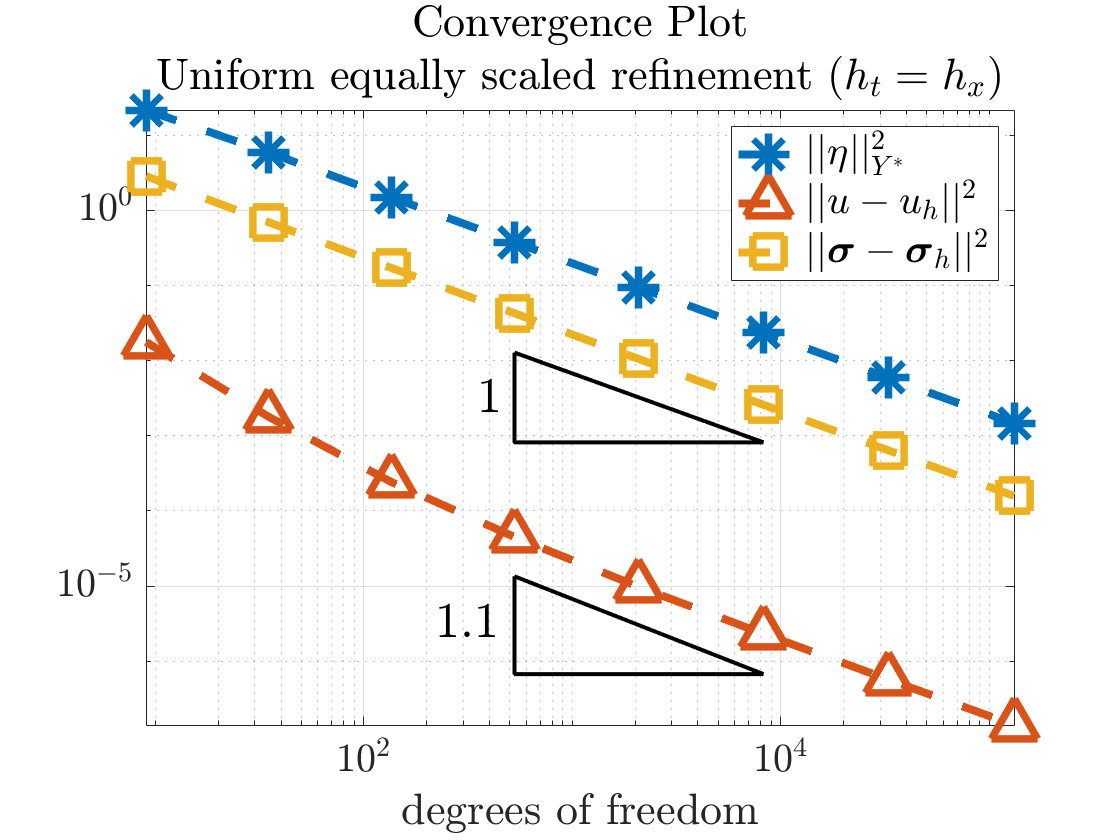
\includegraphics[width = .496\linewidth]{error(un-np)a_10b_-2c_pi.png}
        %\caption{Uniform Mesh}
    \end{subfigure}%
    \begin{subfigure}
        \centering
        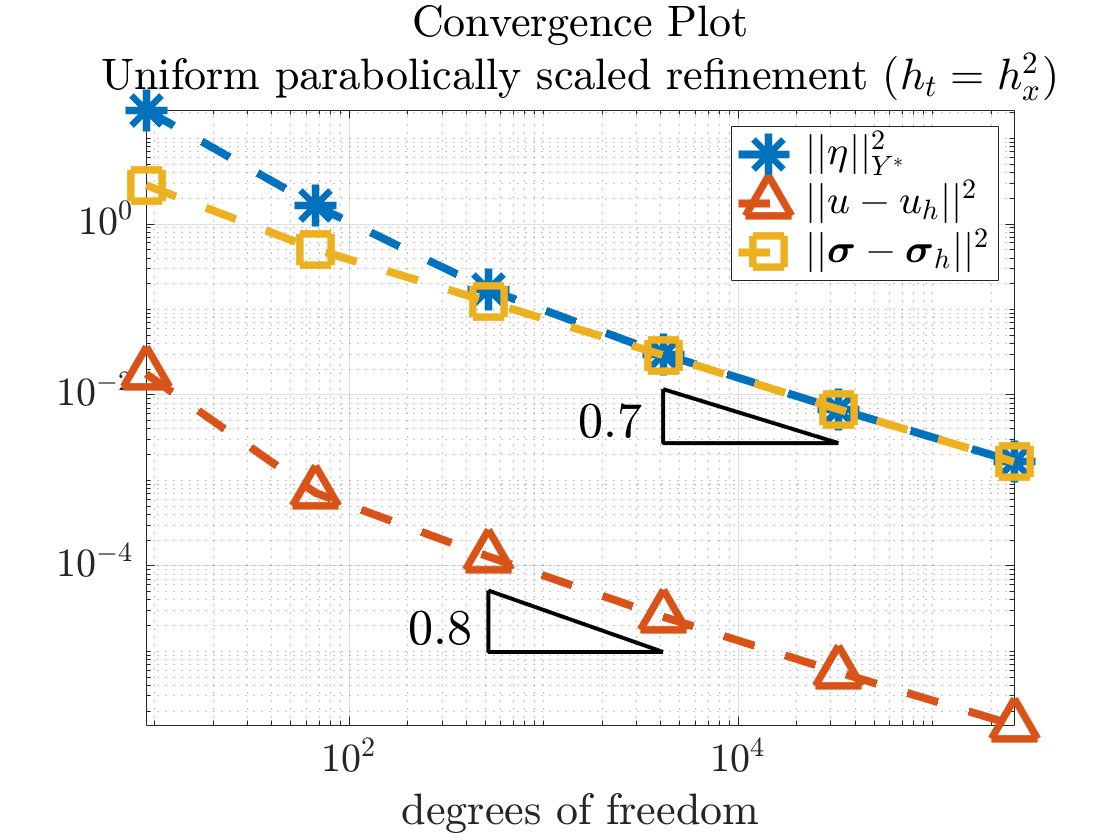
\includegraphics[width = .496\linewidth]{error(un-p)a_10b_-2c_pi.png}
        %\caption{Approximated solution}
    \end{subfigure}%
    \caption{Square residual and squared errors for Experiment 1.}
    \label{figure1}
\end{figure}


\newpage

\subsection{Experiment 2 (Constant initial data).}

In this experiment, we set the constants as $a=2$ and $b=c=1$, the initial data read as $u_0(x)=1$ and the right-hand side as $f(t,x)=0$, for all $(t,x)\in\cyl$. Figure \ref{figure2} shows the residuals from different scenarios as equally and parabolically mesh refinement, and uniform and adaptive refinement for each case. Figure \ref{figure3} shows the approximation $u_h$ and the mesh constructed via adaptive refinement with  a parabolically scaled mesh.

\begin{figure}[ht]
    \centering
    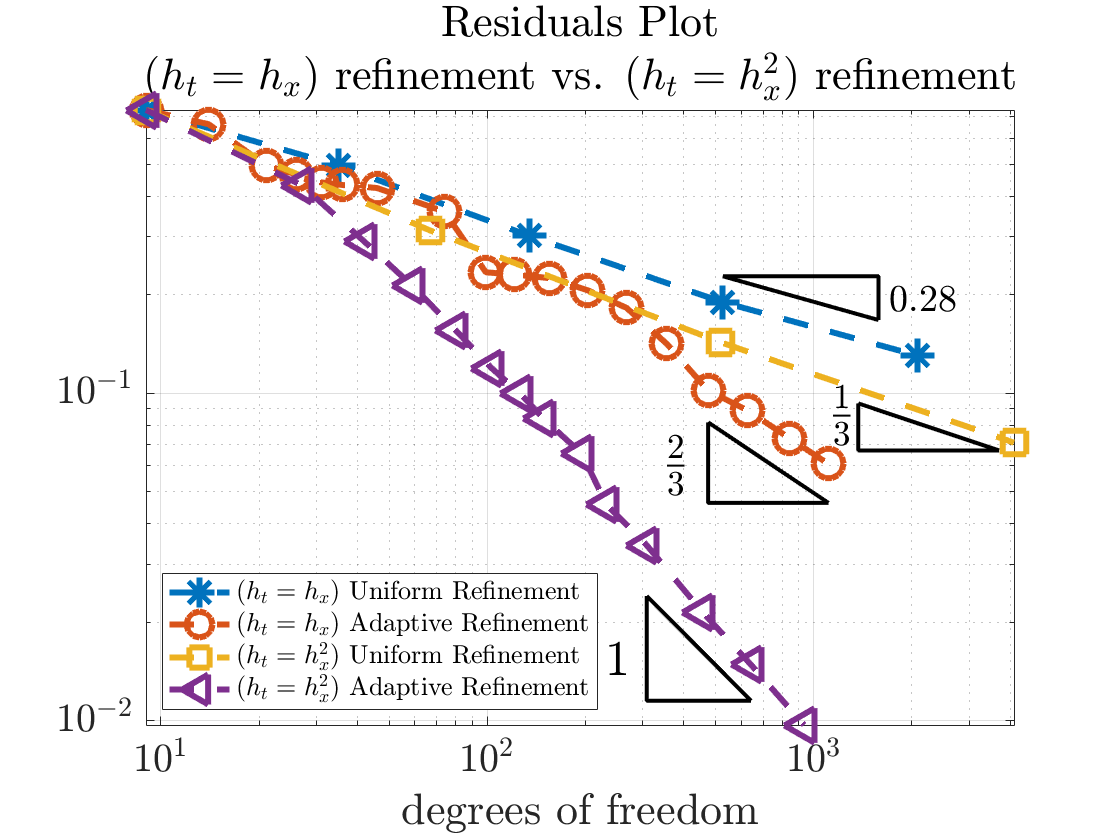
\includegraphics[width = 10 cm]{ResidualsConstant.png}
    \caption{Convergence history plot for the residuals (Experiment 2).}
    \label{figure2}
\end{figure}

\begin{figure}[ht]
    \centering
    \begin{subfigure}
        \centering
        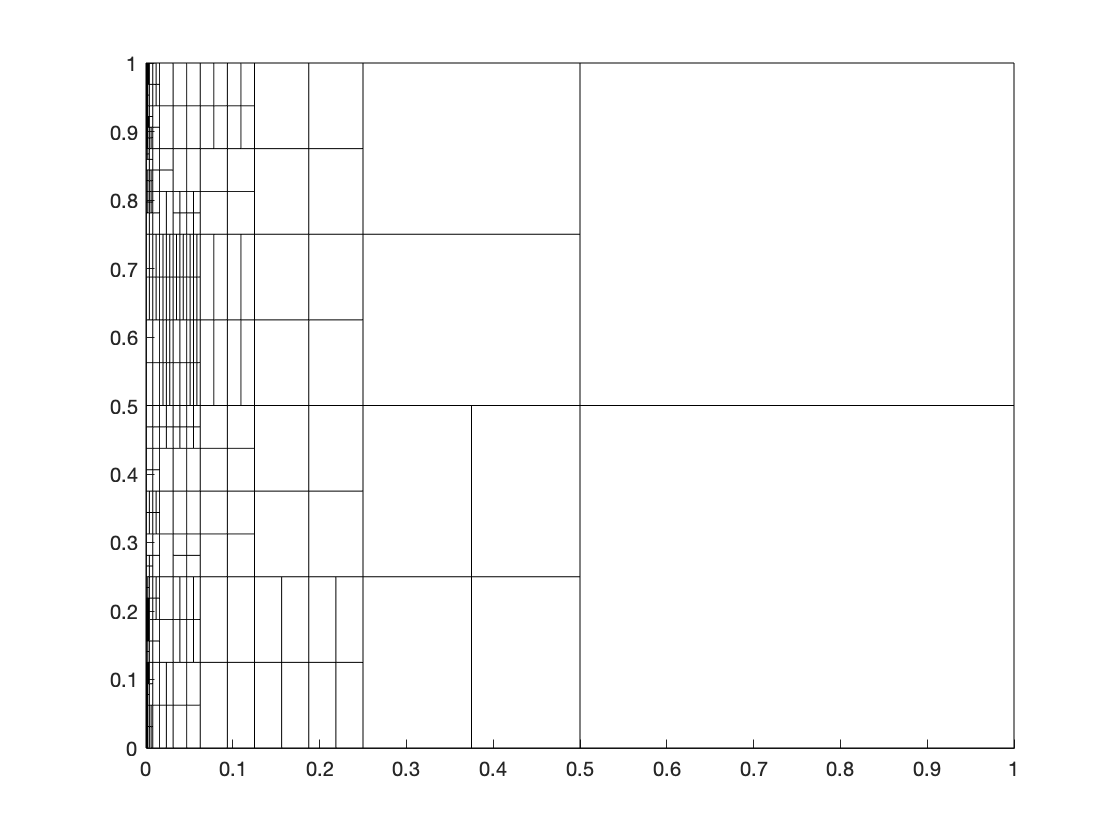
\includegraphics[width = .45\linewidth]{ConstantAdpativeParabolicMesh.png}
        %\caption{Uniform Mesh}
    \end{subfigure}%
    \begin{subfigure}
        \centering
        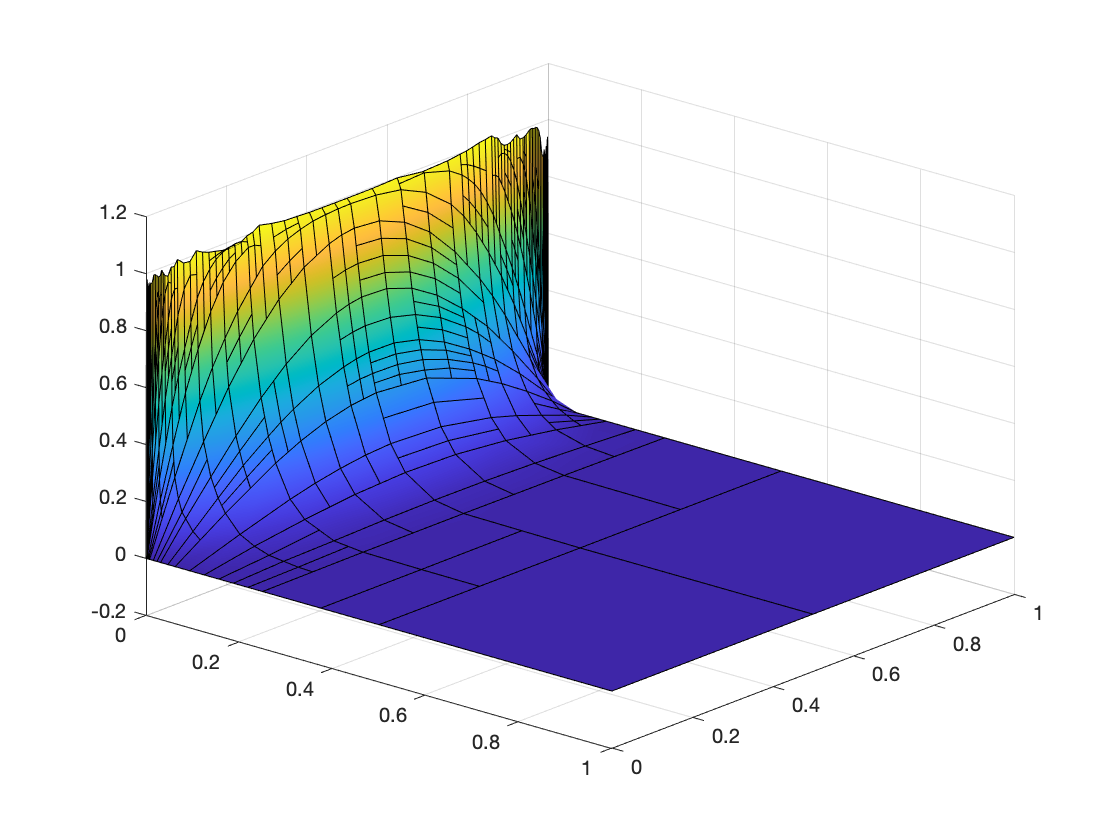
\includegraphics[width = .5\linewidth]{ConstantAdpativeParabolic.png}
        %\caption{Approximated solution}
    \end{subfigure}%
    \caption{A DPG approximation with adaptive mesh and parabolically scaled mesh (Experiment 2).}
    \label{figure3}
\end{figure}

\newpage

\subsection{Experiment 3 (Irregular Initial Data).}


For this experiment we still using the same constants and $f(t,x)=0$, but the initial data read as

$$u_0(x)=\left\{\begin{matrix}
    -1&\text{for }x<1/2,\\1&\text{else}
\end{matrix}\right..$$

As in Experiment 2, Figure \ref{figure4} shows the residuals and Figure \ref{figure5} the approximation $u_h$ and it mesh. 

\begin{figure}[ht]
    \centering
    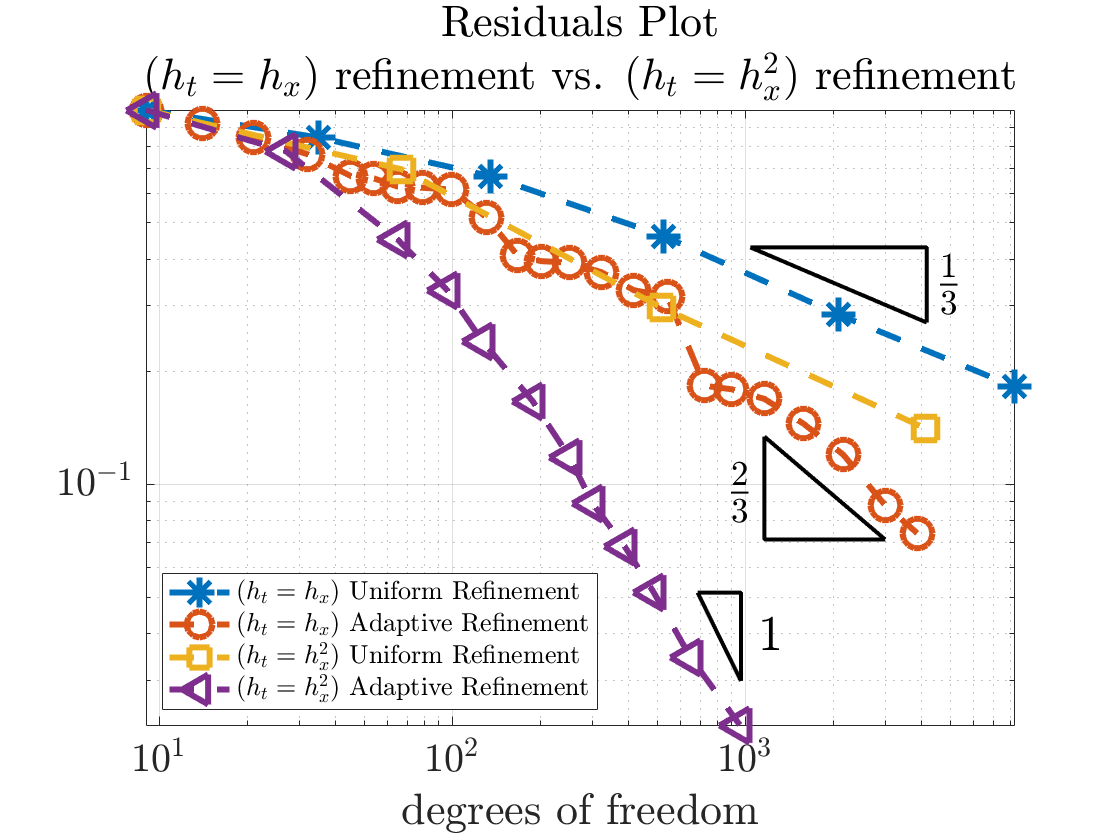
\includegraphics[width = 10 cm]{ResidualsIrregularInitialData3.png}
    \caption{Convergence history plot for the residuals in Experiment 3.}
    \label{figure4}
\end{figure}

\begin{figure}[ht]
    \centering
    \begin{subfigure}
        \centering
        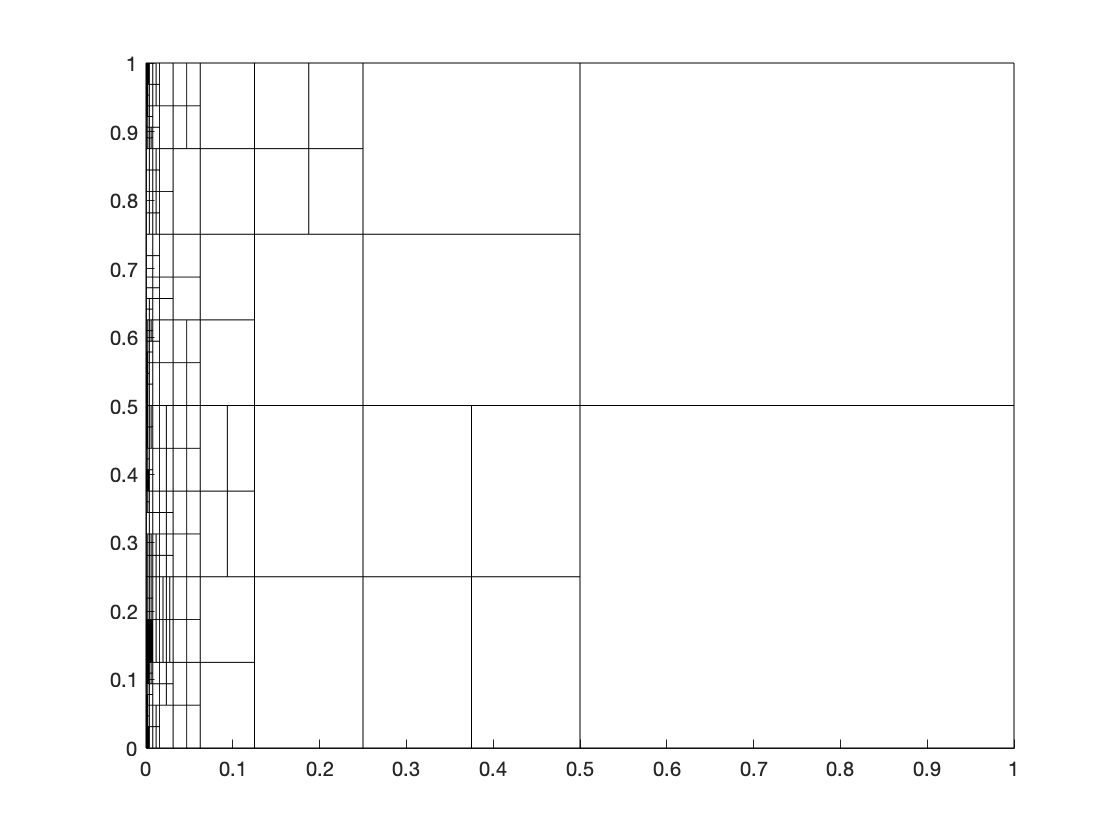
\includegraphics[width = .45\linewidth]{IrregularAdaptiveParabolicMesh.png}
        %\caption{Uniform Mesh}
    \end{subfigure}%
    \begin{subfigure}
        \centering
        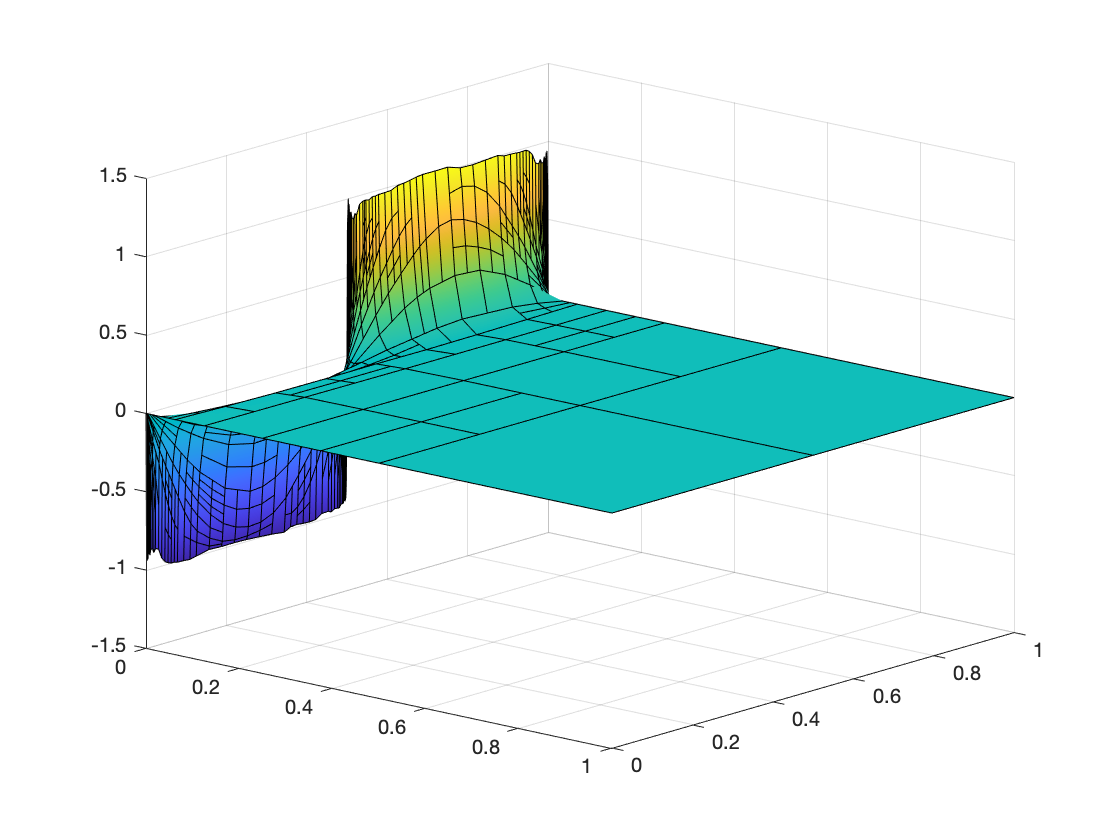
\includegraphics[width = .5\linewidth]{IrregularAdaptiveParabolic.png}
        %\caption{Approximated solution}
    \end{subfigure}%
    \caption{A DPG approximation with parabolic and adaptive mesh refinement (Experiment 3).}
    \label{figure5}
\end{figure}




%\end{comment}
